\documentclass{article}
\usepackage[utf8]{inputenc}
\usepackage{url}
\usepackage[colorlinks=true, allcolors=blue]{hyperref}
\usepackage[a4paper, total={157mm, 240mm}]{geometry}

\title{\Huge Urban Air Pollution Prediction \\
\Large An approach using different deep learning architectures}

\author{\href{mailto:kstroemel@uos.de}%
{Konstantin Strömel}, \href{mailto:tdarius@uos.de}%
{Tjark Darius}, \href{mailto:jclaassen@uos.de}%
{Johannes Claassen}}

\date{March 2022}

\usepackage{natbib}
\usepackage{graphicx}

\begin{document}

\maketitle

\section{Introduction}
In 2018 the World Health Organisation discovered that 90\% of the world's population is suffering from polluted air and that every year around 7 million people die because of air pollution. The WHO states that it is a critical factor in many serious health problems such as lung cancer, strokes and heart diseases. Air pollution causes around one quarter of the total adult deaths through these non-communicable, chronic diseases  \citep{who_air-pollution}.
And even though poor air quality makes respiratory diseases like  COVID-19 more dangerous \citep{iqair_empowering}, the current pandemic also showed that during the lockdown in 2020 84\% of the countries worldwide experienced better air quality than in the previous year \citep{cnn_pandemic-air-quality}.
So human related emissions can directly influence the air quality and our project is trying to examine these influential factors as well as implementing a model that can predict air quality based on satellite data, instead of costly and time intensive  ground-based sensors. This will potentially enable air quality monitoring and management also for low-income countries in Asia and Africa, where most of the pollution related deaths occur. Figure \ref{fig:monitoring} shows an overview of the distribution of monitoring stations. Especially in South America and on the African continent there are very little ground-based measurements. Satellite data could close this big gap in the global monitoring network. \\
\\
\\
\begin{figure}[htb!]
\centering
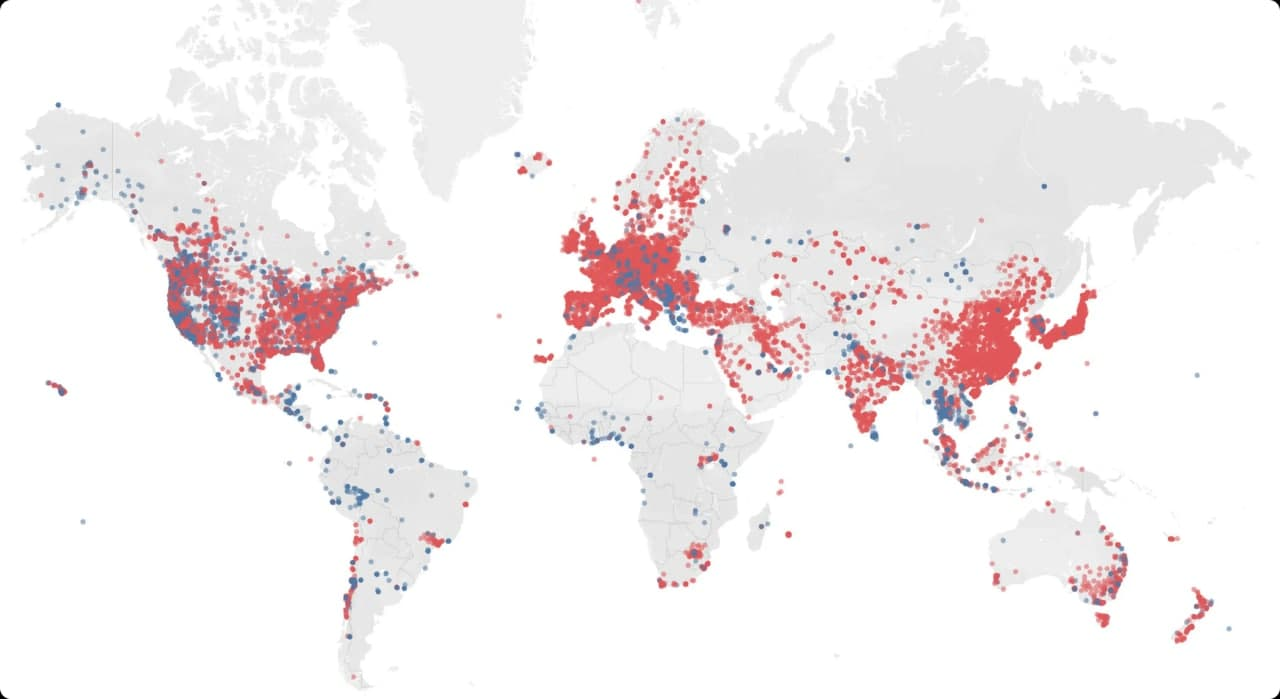
\includegraphics[scale=0.85]{PM2.5_monitoring_stations.jpg}
\caption{Overview of monitoring stations \citep{iqair_empowering}}
\label{fig:monitoring}
\end{figure}

\newpage
\section{Task}
Our goal is to predict the PM$_{2.5}$ score for different cities across the globe based on weather and satellite data \citep{noauthor_zindiweekendz_nodate}.
The PM$_{2.5}$ score refers to atmospheric particulate matter with a diameter of less than 2.5 micrometers in micrograms per cubic meter air ($\mu g / m^3$). It is one of the most widespread air pollutants, consisting of a mixture of solid and liquid particles suspended in the air. Figure \ref{fig:pm25_size} shows how small PM$_{2.5}$ particles are compared to a human hair or a grain of sand \citep{us_epa_particulate_2016}. \\

\begin{figure}[htb!]
\centering
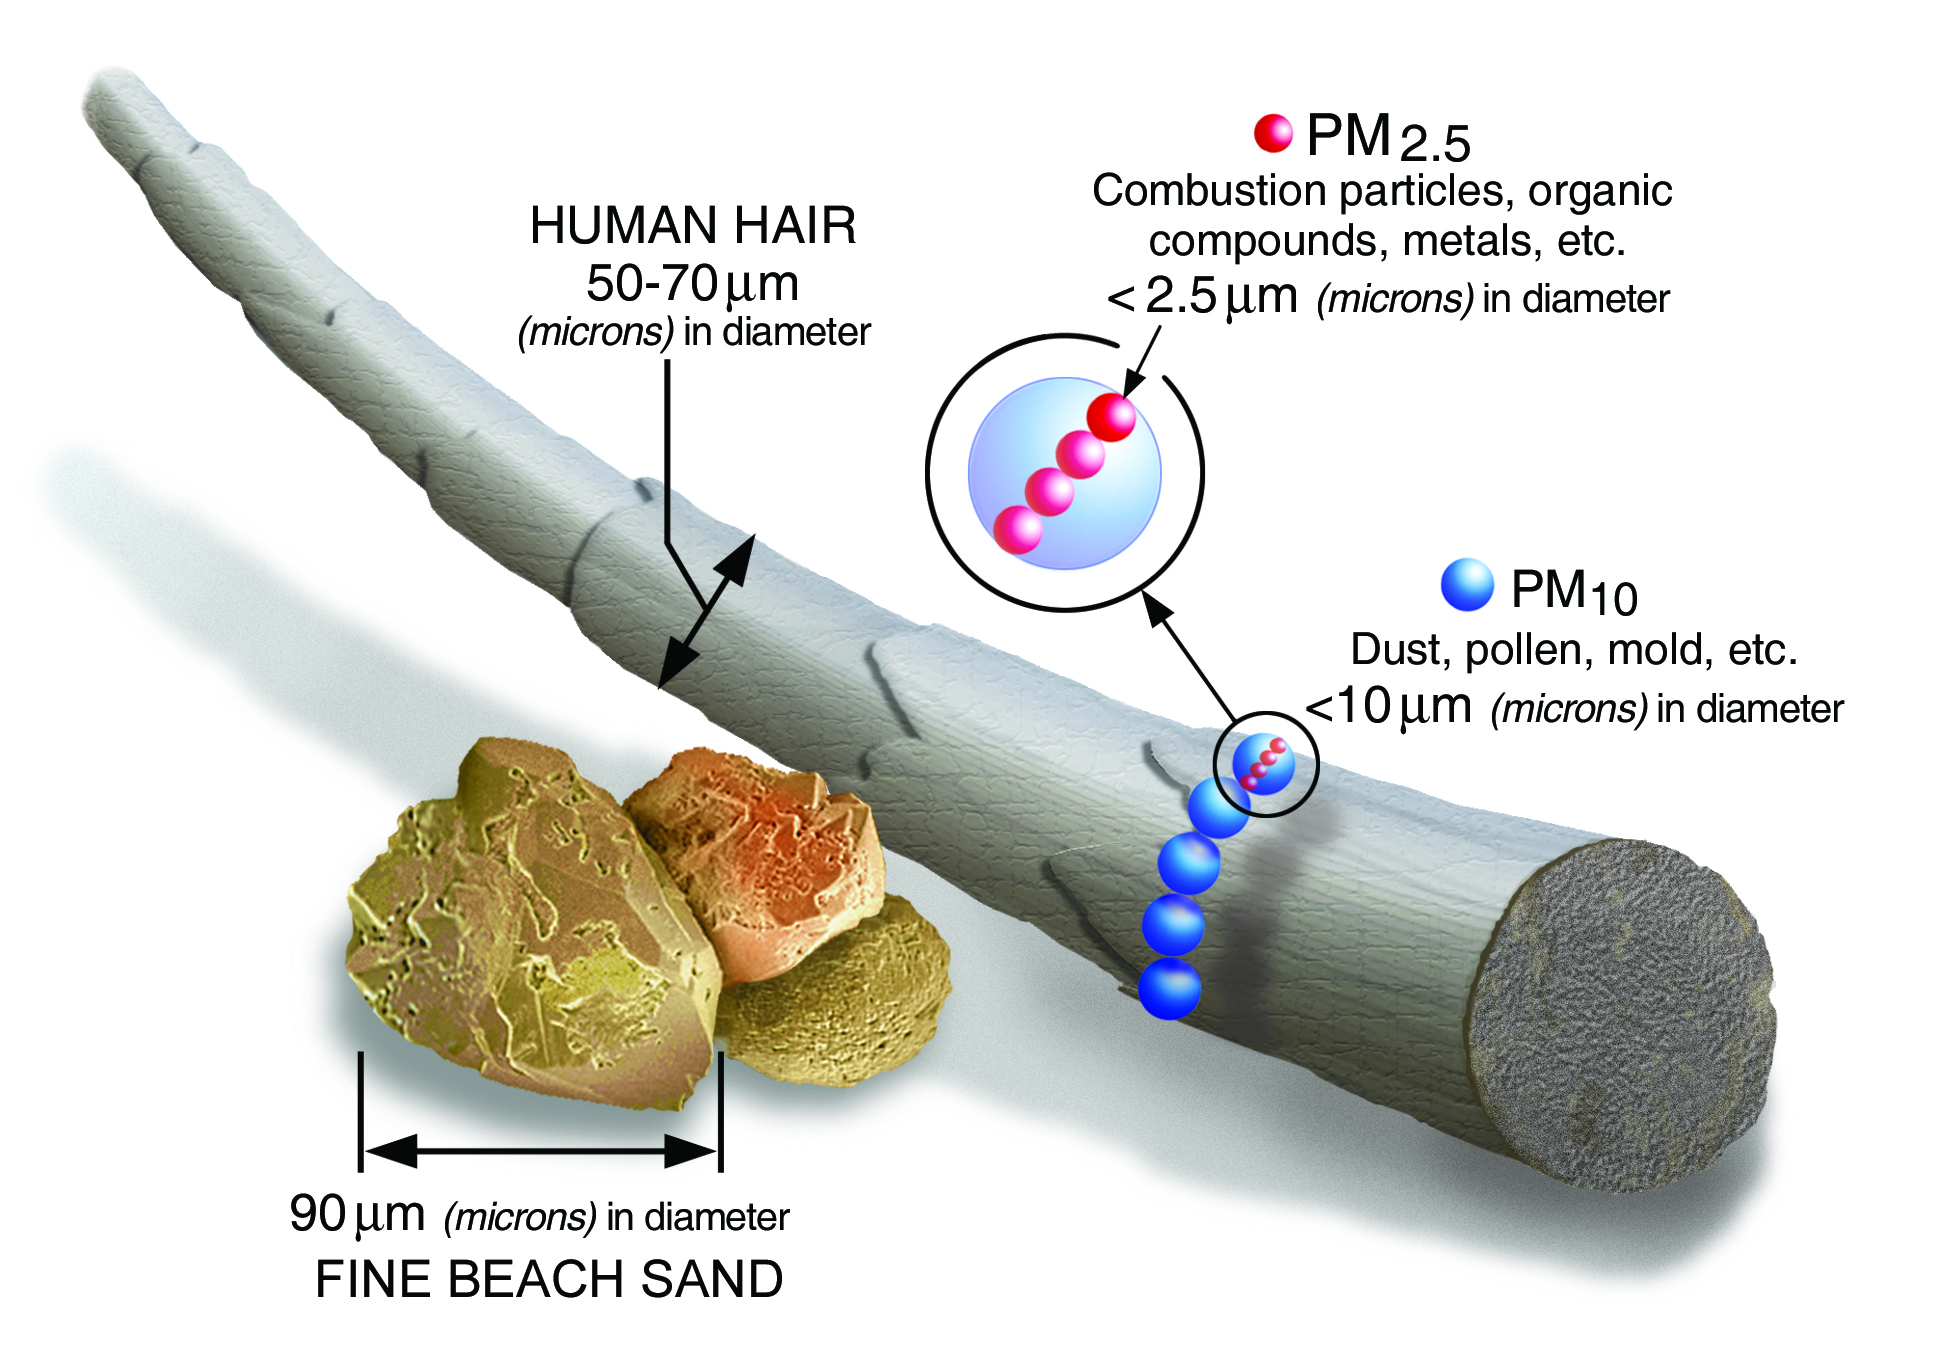
\includegraphics[scale=0.5]{pm25}
\caption{PM$_{2.5}$ particles size comparison \citep{us_epa_particulate_2016}}
\label{fig:pm25_size}
\end{figure}
The score ranges from 0 to 50 $\mu g / m^3$ per 24 hours. The table in figure \ref{fig:pm25} shows the WHO guidelines for PM$_{2.5}$ pollution. It also serves as a color code for the global PM$_{2.5}$ map in figure \ref{fig:pm25_map} \citep{iqair_empowering}.  \\

\begin{figure}[htb!]
\centering
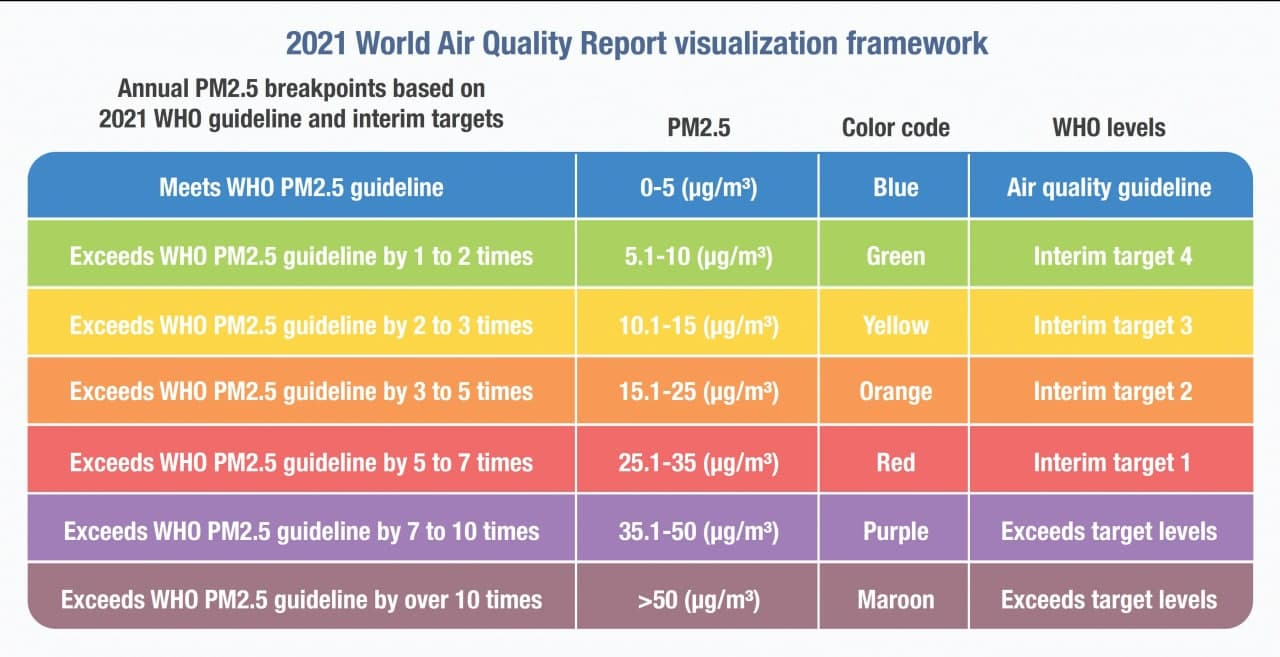
\includegraphics[scale=0.8]{WHO_guidelines.jpg}
\caption{WHO PM$_{2.5}$ guideline \citep{iqair_empowering}}
\label{fig:pm25}
\end{figure}

\begin{figure}[htb!]
\centering
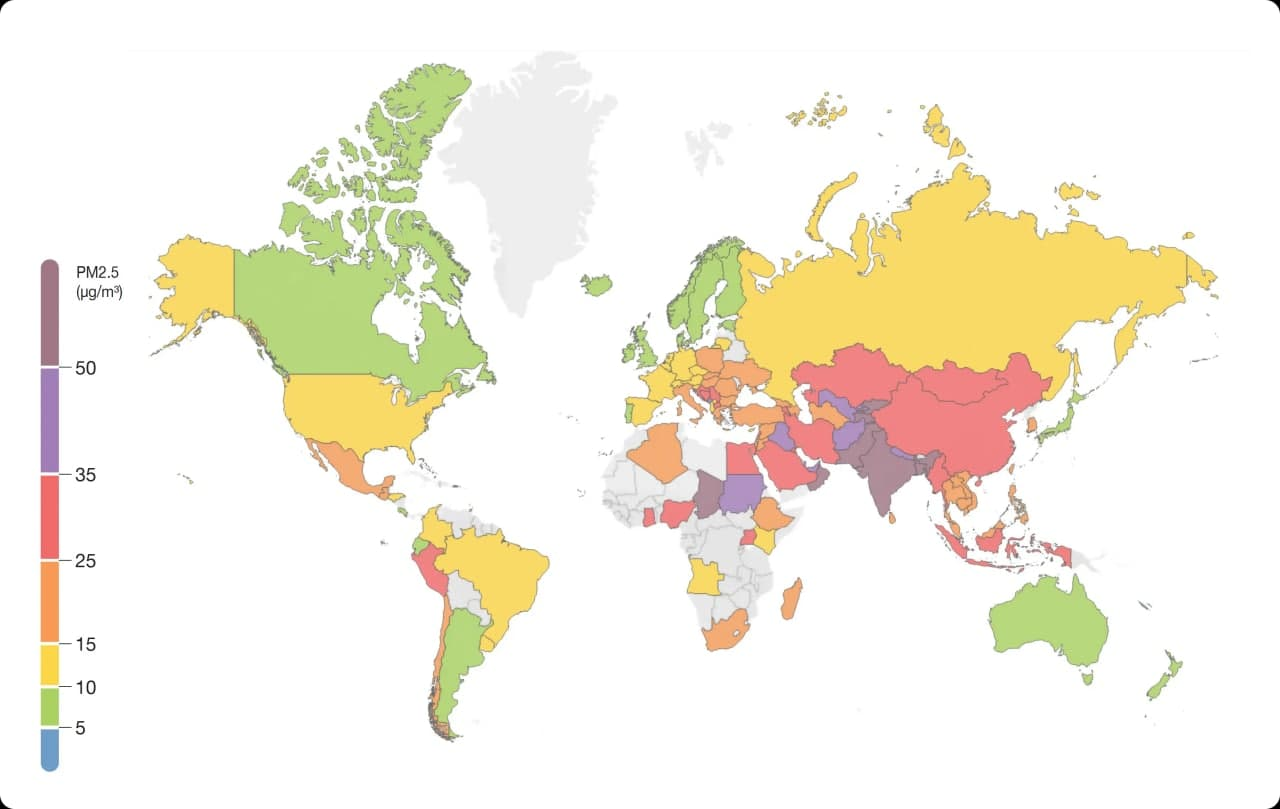
\includegraphics[scale=0.8]{global_PM2.5_map.jpg}
\caption{Global PM$_{2.5}$ map \citep{iqair_empowering}}
\label{fig:pm25_map}
\end{figure}
For this task we had to solve a so-called "out of distribution" problem, because we had to predict target values for cities that were not part of the training data. 
In the following section we will describe the available training data and how we used it for our model. 
\newpage
\section{\href{https://github.com/tjayada/iANNwTF_Project/tree/main/data/raw\%20data}{Data}}
The data provided by \textit{Zindi} comprises of three different main sources of data. First, the target values, which are five columns in total, are obtained from ground-based air quality sensors. Second, there are six columns of general weather data produced by the Global Forecast System\footnote{for more information refer to https://nomads.ncep.noaa.gov/txt\_descriptions/GFS\_doc.shtm}, operated by the U.S. National Weather Service. And third, there are in sum 68 columns of satellite data, provided by the Sentinel-5 Precusor\footnote{for more information refer to https://sentinel.esa.int/web/sentinel/missions/sentinel-5p} project.

\subsection{Target data}
The column {\fontfamily{qcr}\selectfont target} displays the PM$_{2.5}$ particle concentration, which describes the concentration of fine particles of diameter less than 2.5 $\mu$m. These are of great public interest due to their health impact  \citep{tai_meteorological_2012}.
The remaining four target columns (namely {\fontfamily{qcr}\selectfont target\_min}, {\fontfamily{qcr}\selectfont target\_max}, {\fontfamily{qcr}\selectfont target\_variance} and {\fontfamily{qcr}\selectfont target\_count}) are summary statistics of the target variable for each entry.

\subsection{Weather data}
As mentioned, the weather data is obtained from the \textit{Global Forecast System}. This is no measured data but predicted data produced by the FV3 model developed by the U.S. National Weather Service. Since we use data from January 2020 to April 2020, the model ran in version 15.2  \citep{emc_gfs_17-03-2022}.\\
The model output consists of nine variables of which six are used in the data set.
{\fontfamily{qcr}\selectfont precipitable\_wa-ter\_entire\_atmosphere} describes the amount of water that is precipitable for the whole atmosphere in $kg/m^2$, {\fontfamily{qcr}\selectfont relative\_humidity\_2m\_above\_ground} gives the relative air humidity in percent at two meters height, 
{\fontfamily{qcr}\selectfont specific\_humidity\_2m\_above\_ground} refers to the mass of water in a specific amount air in $kg/kg$, {\fontfamily{qcr}\selectfont temperature\_2m\_above\_ground} gives the air temperature at two meters height, {\fontfamily{qcr}\selectfont u\_component\_of\_wind\_10m\_above\_ground} describes the $u$-component of the wind, i.e., the vector showing the wind direction between east and west and {\fontfamily{qcr}\selectfont v\_component\_of\_wind\_10m\_a-bove\_ground} giving the $v$-component, i.e., the wind direction in terms of north or south \citep{google_gfs_17-03-2022}.

\subsection{Satellite data}
The satellite data is gathered by the Copernicus Sentinel-5 Precursor mission, conducted by a collaboration of the European Space Agency (ESA), the European Commission and the Netherlands Space Office. The data is collected by the Tropospheric Monitoring Instrument (TROPOMI) carried by the Sentinel-5P satellite which was launched in October 2017. Its main goal is to perform atmospheric measurements in order to monitor parameters such as air quality, UV radiation or climate change  \citep{esa_sentinel-mission-page_nodate}.
It measures the tropospheric concentration of substances associated with air quality, such as carbon monoxide (CO), formaldehyde (HCHO), ozone (O$_3$), sulphur dioxide (SO$_2$), nitrogen dioxide (NO$_2$) and those associated with climate forcing, for instance methane (CH$_4$) and water vapour (H$_2$O) \citep{esa_thematic_nodate}. \\
As mentioned, the satellite data consists of 68 columns covering the substances NO$_2$, O$_3$, CO, HCHO, H$_2$O (i.e., clouds), SO$_2$, CH$_4$ and the UV Aerosol Index\footnote{for more information refer to http://www.tropomi.eu/data-products/uv-aerosol-index}. \\
For instance, the data set contains twelve columns for NO$_2$ (starting with {\fontfamily{qcr}\selectfont L3\_NO2\_}). Four of these variables are actual measurements about NO$_2$. {\fontfamily{qcr}\selectfont column\_number\_density} displays the vertical column density of NO$_2$ divided by the total air mass factor for the whole atmosphere. \\ {\fontfamily{qcr}\selectfont tropospheric\_NO2\_column\_number\_density} and \\ {\fontfamily{qcr}\selectfont stratospheric\_NO2\_column\_number\_density} show the same just for the troposphere and stratosphere, respectively. \\ {\fontfamily{qcr}\selectfont NO2\_slant\_column\_number\_density} refers to the slant column density.\footnote{For more information on density measures, refer to https://sentinels.copernicus.eu/web/sentinel/technical-guides/sentinel-5p/level-2/doas-method} Besides that, there are a few columns delivering meta data about the measurements.
{\fontfamily{qcr}\selectfont sensor\_altitude},  {\fontfamily{qcr}\selectfont sensor\_azi-muth\_angle}, {\fontfamily{qcr}\selectfont sensor\_zenith\_angle}, {\fontfamily{qcr}\selectfont solar\_azimuth\_angle} and  {\fontfamily{qcr}\selectfont solar\_zenith\_angle} refer to the position and angle of the sensor and the sun, respectively. \citep{noauthor_sentinel-5p_nodate}

\subsection{Data preprocessing}
The provided training data described above has 30557 entries in total, spanning over 82 features. Only 12 of these features have no missing values while the other features range between missing a couple hundred values to over 24000. \\
Simply removing each entry, which contains a missing value would result in a data set with only 3915 entries left. So to solve this problem of missing values we came up with two possible solutions:

\subsubsection{\href{https://github.com/tjayada/iANNwTF_Project/blob/main/data\%20preparation/05_finished_and_clean(1).ipynb}{Remove features with most missing values}}
The first approach is based on the fact that most features contain more than 23000 complete entries and only a couple features have more than 80 \% of their data missing. So the idea is to exclude these mainly incomplete features and afterwards remove the entries with missing data. This results in a data set where the columns detailing methane (CH$_4$) concentration and respective satellite meta data are removed entirely. After removing individual entries with missing data, the data set then has 18219 entries in total spanning over 75 features.

\subsubsection{\href{https://github.com/tjayada/iANNwTF_Project/blob/main/data\%20preparation/05_finished_and_clean(2).ipynb}{Fill in all missing values}}
The second approach is trying to use all the data we are provided with as best as possible. So we calculated the mean of each feature and then replaced missing values with the respective mean value. This method is somewhat questionable, since some features consist of mainly missing data, but we were interested how our models would perform on each of these two data sets.\\
The results showed that all models performed marginally better on the data set with the removed methane columns than on the data set with filled in mean-values.

\subsubsection{Adding and removing features}
Independent of the approach we used for the missing values, we also added some features relating to dates and times. Since the dates were provided in the data set, we then used this information to add a feature that tells us what weekday the date is, whether the given date is on a weekend or not, which month and season it belongs to and what day of the year the provided date is. With these new features we then could remove the features that we could not use based on the object types, which were the Place IDs and Dates. \\ 
After normalizing the data set using the MinMaxScaler from the Sklearn library\footnote{https://scikit-learn.org/stable/modules/generated/sklearn.preprocessing.MinMaxScaler.html} 
we used Principal Component Analysis (PCA)\footnote{https://scikit-learn.org/stable/modules/generated/sklearn.decomposition.PCA.html} 
to determine which features are considered important for the variance of the data set and thus useful to add previous time steps to the data set. In total six features were found to be responsible for more than 75\% of the data sets variance. These six features were then added to the data set with a shift of one, such that each data point would have the information for these six features of the previous day as well. It would have been possible to add the data of more than one day, for example a whole week previous to the given data points date, but since the data set has many different locations, these shifts would end up adding data of previous days to locations that are possibly independent of each other. So to not mix up different locations with each other, while still getting the benefit of these useful previous features, we decided to only shift by one day.

\subsubsection{\href{https://github.com/tjayada/iANNwTF_Project/blob/main/data\%20preparation/06_finished_and_clean_LSTM(1).ipynb}{Special LSTM data with encoded Place\_ID}}
Lastly we have created a special LSTM data set which is based on the first data set, which excluded the methane columns, but instead of removing the locations, we actually encoded the 
{\fontfamily{qcr}\selectfont Place\_ID} feature, so each location is given a unique natural number.This enables the LSTM to use this information. To do this encoding we converted the anonymous {\fontfamily{qcr}\selectfont Place\_ID} feature into unique categories, and then gave each category a different natural number to represent the location.

\section{Related work}
In this section we will review previous studies on air quality prediction by researchers, who employed different deep learning techniques. 
Ong, Sugiura and Zettsu proposed a deep recurrent neural network (DRNN) specifically designed for PM$_{2.5}$ prediction. Their network is improved by a novel dynamical pre-training method. They use stacked autoencoders to build up their RNN. In this concatenation of autoencoders the output of the model of the layer below serves as input for the next autoencoder. Due to that each hidden layer is a higher-level abstraction of the previous layer, therefore the last hidden layer contains the high-level structure and representative information of the input.
This results in the big advantage that the network can select relevant sensors for its predictions. They achieve this through a regularized regression technique called elastic net (EN). The training data is often quite sparse and incomplete. Through the EN they were able to filter out sensors, that did not improve the predictions significantly. This reduces the overall computational costs and results in a more interpretable response–predictor relationship \citep{ong_dynamically_2016}.

In 2019 Wen et al. developed a novel neural network arcitecture for air pollution prediction. It is a combination of a convolutional neural network (CNN) and a long short-term memory (LSTM) network. In figure \ref{fig:c_lstm} their C-LSTM model is sketched out. They argue that this combination is beneficial due to the combination of temporal and spatial features in the training data \citep{wen_novel_2019}.

\begin{figure}[htb!]
\centering
\includegraphics[scale=1.25]{C_LSTM model.jpg}
\caption{C-LSTM model \citep{wen_novel_2019}}
\label{fig:c_lstm}
\end{figure}
Chae et al. used an interpolated convolutional neural network (ICNN) for their predictions of air pollution in South Korea. CNNs work best with an evenly spaced grid like data. To achieve this spatially balanced structure they made use of interpolation. The pollution monitoring stations are concentrated in bigger cities with unequal distances between the stations. They created an equally spaced empty grid and filled in data points as if a virtual measuring station was located at every grid point through interpolation from the existing measurements \citep{chae_pm10_2021}. Figure \ref{fig:icnn} visualizes their network architecture.

\begin{figure}[htb!]
\centering
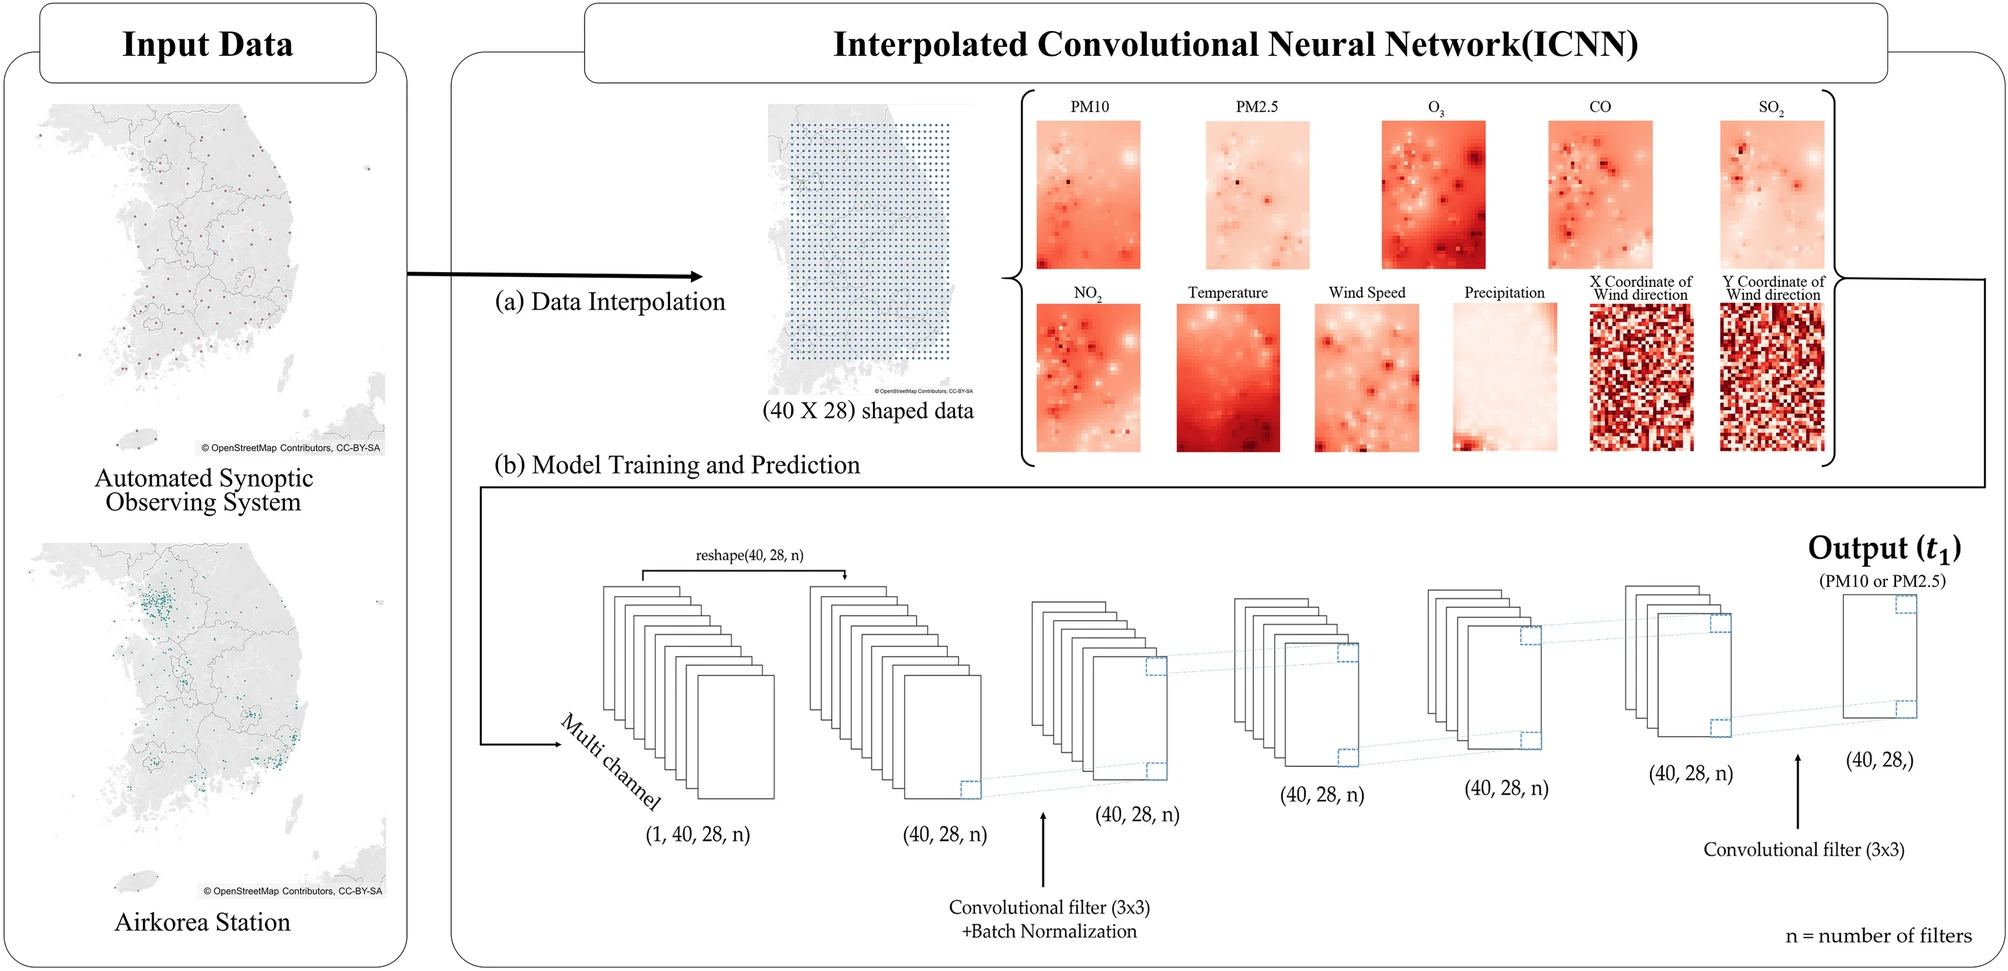
\includegraphics[scale=0.22]{ICNN.jpg}
\caption{ICNN model \citep{chae_pm10_2021}}
\label{fig:icnn}
\end{figure}
\section{Model}
Due to the chronologically ordered data we believe a LSTM is the best choice for predicting the desired targets. Since these Long Short-Term Memory models are also being actively used for time series forecasting like the weather or stock markets, so it makes sense to use them for our temporally structured data as well. This special kind of Recurrent Neural Network would be perfect, if the data did not include over 300 different locations and if the target locations we wanted to predict were part of the training data, but the locations in the training data set and the locations for the predictions are entirely different from each other. This problem led us to try multiple models that could disregard the chronological order and different locations by only using the weather and satellite data itself. As mentioned in the Data preprocessing section, we have included the data of the six most important features of the previous data points date and thus managed to include this information without the data being necessarily chronologically ordered. \\
We always used the same hyperparameter, error function and optimizer to be able to compare the different model structures better. We used a training loop with 100 epochs, the Mean Squared Error function and the Adam optimizer with a learning rate of 0.01 for all models.
The four different models we used are:
\subsection{\href{https://github.com/tjayada/iANNwTF_Project/blob/main/model/06_finished_linear_regression/06_finished_linear_regression(1).ipynb}{Linear Regression} }
The first and  most simple idea is to use a linear regression model to predict the target values. To our surprise the linear regression model performed rather well with a Root Mean Squared Error (RMSE) of 37.6 for both data sets. \\
As the name may suggest this model only has one layer and one unit with a linear activation function, but this simple structure was not that much worse than the next model we used, which was a Multi-Layer Perceptron (MLP).
\subsection{\href{https://github.com/tjayada/iANNwTF_Project/blob/main/model/07_finished_mlp_regression/07_mlp_regression(1).ipynb}{MLP}}
The MLP is a better fit for our problem, since the complex data is most likely not best described through a single linear function, but rather multiple (non-)linear functions. So the input layer has as many units as our data features, which is either 78 for the first data set without the methane columns or 85 features for the data set with the mean filled missing values. These input layer units have a linear activation function, while the next three hidden layers use a rectified linear activation function. These hidden layers double each time in unit size, so the first on has 160, then 320 and then 160 again. The output layer has again only one unit, since we only want to predict one value, with a linear activation function. We got a RMSE of 30.6 for the first data set and a RMSE of 33.3 for the second one. As mentioned in the data preprocessing section, all models performed slightly better on the first data set. The next model we tried was a Convolutional Neural Network (CNN).

\subsection{\href{https://github.com/tjayada/iANNwTF_Project/blob/main/model/08_finished_CNN_regression/08_CNN_regression(1).ipynb}{CNN}}
The CNN is the first unconventional model for this kind of task. To be able to use the CNN we need to add an extra empty dimension to our data, so the shape is then 
{\fontfamily{qcr}\selectfont (number\_of\_entries, number\_of\_features, 1)}. The CNN itself consists of five 1-dimensional convolutional layers (also called temporal convolution) starting with 32 filters and then doubling for each layer up to 128 filters in the third layer and then halving again back to 32 filters in the fifth layer. The kernel size 2 and the ReLU activation function stay the same across each layer. Then we flatten the input and use simple dense layers for the output. We are able to get a RMSE of 31.9 for the first data set and a RMSE of 33.8 for the second data set.

\subsection{\href{https://github.com/tjayada/iANNwTF_Project/blob/main/model/10_finished_basic_LSTM_regression.ipynb}{LSTM}}
Lastly we used a Long short-term memory (LSTM) network architecture, which we deemed the most promising model for this problem and data. We implemented our \href{https://github.com/tjayada/iANNwTF_Project/blob/main/model/11_LSTM_own_implementation.ipynb}{own LSTM} model, but due to time constraints we relied on the functional API of TensorFlow for a comparison model.
The basic LSTM model achieved a RMSE of 30.6, equal to the MLP, for the first data set and the best RMSE so far for the second data set with an error of 31.4 with the same parameters as the other models. \\
But as we think that this is the best approach to our problem, we then tried to optimize its performance. We implemented a model with a LSTM with 300 units and used a dropout layer with a value of 0.5, which means that half the neural connections would be dropped, in response to potential overfitting. Also in response to the overfitting was an early-stopping function used, and at the end a linear dense output layer with 1 unit.
We trained for 1000 epochs and were using the Nadam optimizer with a learning rate of 0.01.
To be able to use the 
{\fontfamily{qcr}\selectfont Place\_ID } 
we have created the third data set that encoded the different locations, but to our surprise the LSTM performed worse with the ordered data that also has locations, even though the LSTM should in theory profit from chronologically ordered data that can be distinguished by different locations. \\
The model has a RMSE of 33.7 for the special shuffled LSTM data set and a RMSE of 40.8 for the special unshuffled LSTM data set. \\
The four different performances of the \href{https://github.com/tjayada/iANNwTF_Project/tree/main/model/09_finished_LSTM_regression}{LSTM models} can be seen in figure 7. The models are divided into shuffled and not shuffled data as well as the data set they were using, either "With location", which is the special LSTM data set based on the first data set without the methane columns or "No location" which is the normal first data set without the methane columns.

\begin{figure}[htb!]
\centering
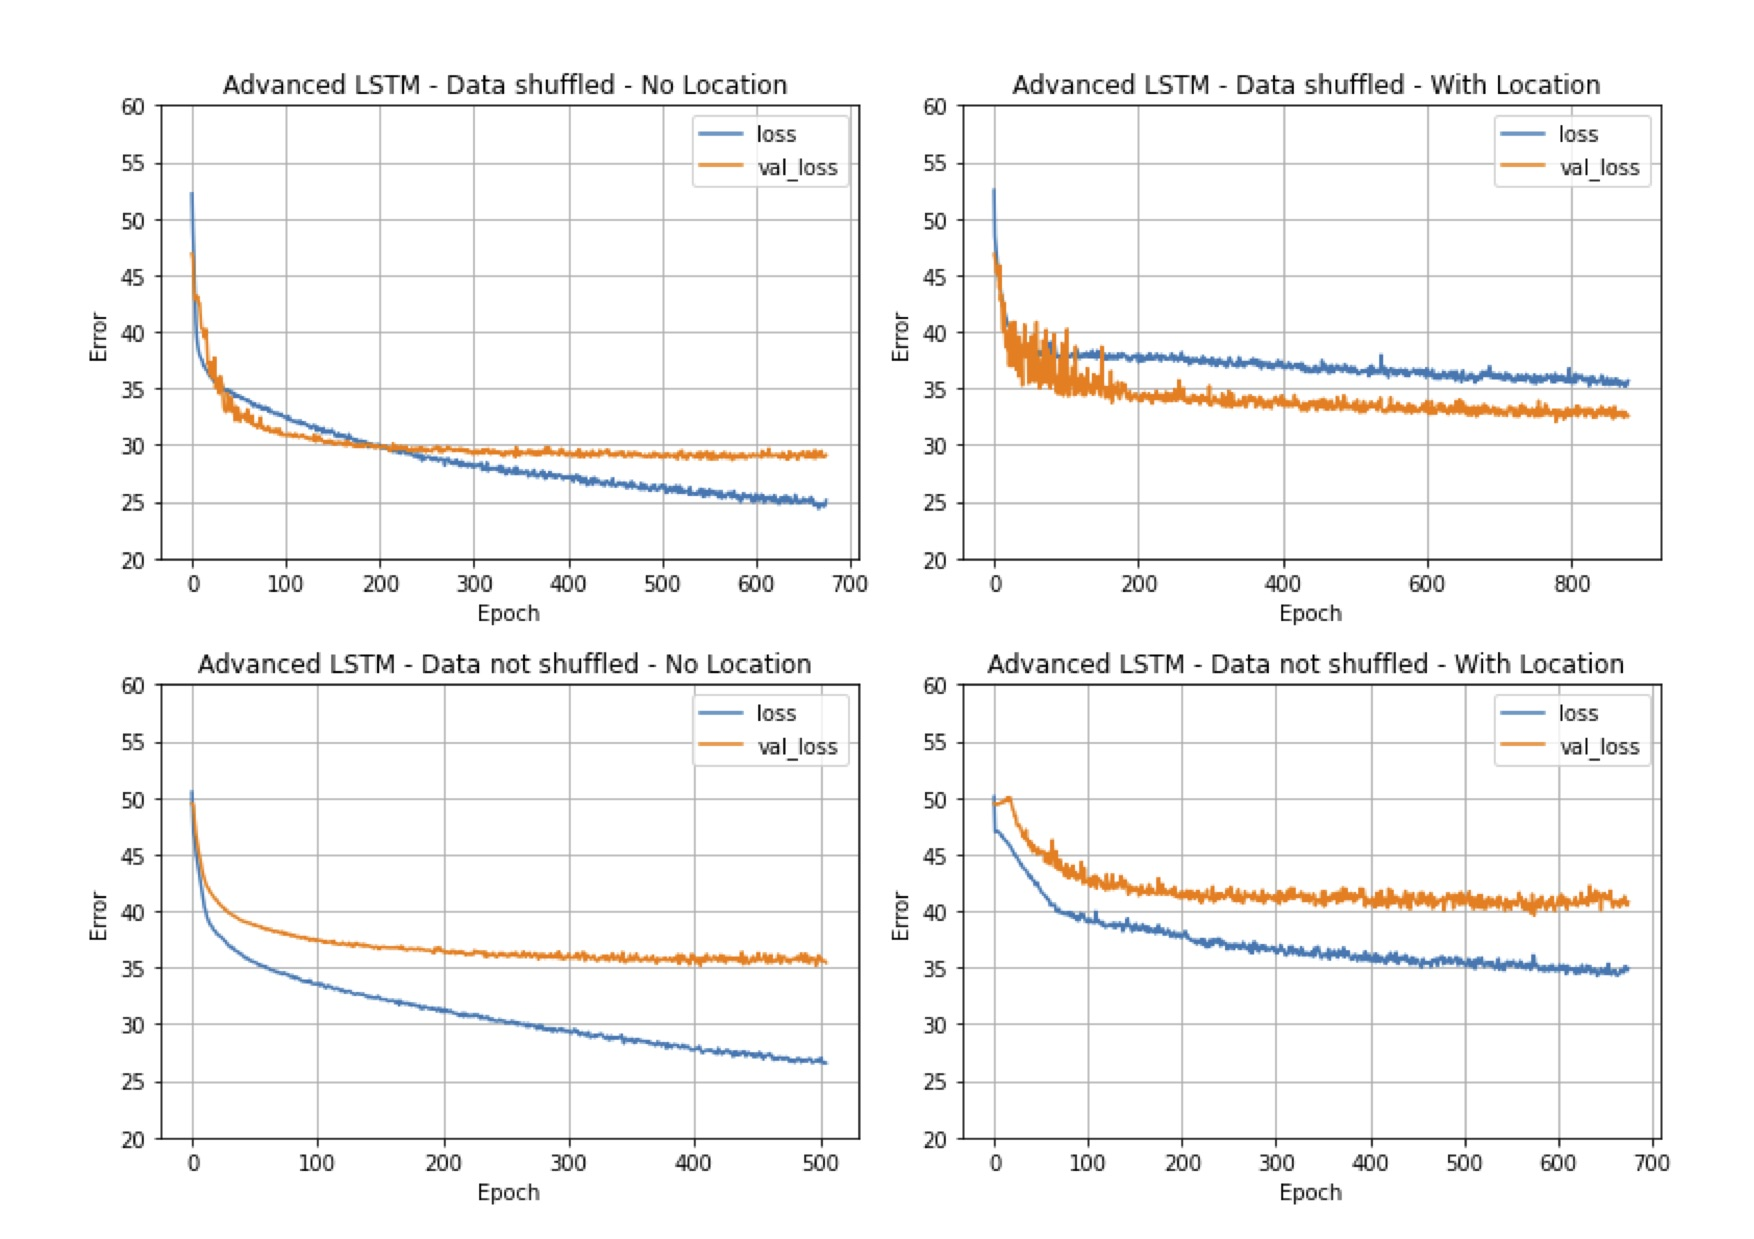
\includegraphics[scale=0.25]{final_comparison.jpg}
\caption{Model comparison}
\label{fig:model_comparison}
\end{figure}
\newpage
\section{Results}
Throughout the paper we already mentioned multiple interesting results. For once we determined that the first data set with the removed methane columns was better suited for training and predictions than the second data set that used the mean to replace missing values. This can most likely be explained by the fact that filling in too many missing values actually changes the data in a way that does not reflect the original data distribution anymore. Another observation was that the MLP and LSTM without locations were the best performing models. For a comparison you can look at Table \ref{table:1}. Loss 1 refers to the Root Mean squared error (RMSE) using the first data set and Loss 2 to the RMSE of the second one. \\
The linear regression model assumes a way too simple data distribution and the CNN model structure is not necessarily build for this regression task with (originally) chronological structured data. Another interesting point is that the LSTM actually performed worse when we added the location data and did not shuffle the data to keep the chronological structure of the data. \\ 
To be able to interpret these results better, we then also used the Mean Absolute Error (MAE) as a metric and got a MAE of about 21 for our advanced LSTM and thus the average prediction error was $\pm$ 21 for the target value. With such an error we are able to distinguish good air quality from unhealthy air quality quite reliable, since good air quality ranges from 0 to 12 PM$_{2.5}$ ($\mu g/m^3$) and unhealthy air quality ranges from 55 to 150 PM$_{2.5}$ ($\mu g/m^3$) per 24 hours.

\begin{table}[h!]
\centering
\begin{tabular}{ |c|c|c|c|c|c| } 
 \hline
 Model & Regression & MLP  & CNN & basic LSTM & advanced LSTM\\ 
 \hline
 Loss 1 & 37.6 & 30.6 & 31.9 & 30.6 & 28.8\\ 
 Loss 2 & 37.6 & 33.3 & 33.8 & 31.4 & / \\ 
 \hline
\end{tabular}
\caption{Comparison of results.}
\label{table:1}
\end{table}

Regarding the data set we found out that certain features are more important in explaining the distribution than others. For example the feature 
{\fontfamily{qcr}\selectfont L3\_SO2\_sensor\_azimuth\_angle }
explains 29\% of the variance of the data set or the fourth most important feature 
{\fontfamily{qcr}\selectfont weekend }
was added artificially by us and explains 8 \% of the data sets variance. And more than $\frac{3}{4}$ of the data sets variance can be explained by only 6 of the around 80 different features.

\section{Outlook}
Due to the limited realm of our project we were not able to employ hyperparameter optimization and test further regularization techniques. In the future another interesting approach would be to use the location {\fontfamily{qcr}\selectfont (Place\_ID) }with an improved encoding, so the LSTM and maybe the other models as well, could profit from this, instead of reducing the performance as we have experienced it. We consciously decided against using the locations for the most part, since we were dealing with an out of distribution problem, so the the locations would have been completely ineffective for the prediction, since they were entirely different for the training and prediction part, but maybe a model might profit from the location, even though it did not work for our simple encoding scheme. Alongside this realization would be an improvement based on the sequential data set an interesting endeavour, since we experienced a worse performance for our LSTM models, when using the unshuffled data.


\section{Conclusion}
Overall we are satisfied with our work, with creating and comparing multiple approaches of different models and analysing the data set thoroughly. \\
We learned that air pollution is a serious problem, which is responsible for many of our challenges regarding health and the environment, which we did not know before working on this problem. We hope that the we can make our readers aware of this problem through our report. Paying attention to these small particles influencing our lives is very important. And we think there is a lot of potential for AI to create solutions to help reduce pollution itself and not only monitor it. \\
\newpage
\bibliographystyle{ieeetr}
\bibliography{references}


\end{document}
